\documentclass{article}
\usepackage{geometry,tikz}
\usetikzlibrary{intersections,backgrounds,positioning}
\usepackage[version=3]{mhchem}
\makeatletter
\tikzset{%
atom/.style={circle,ball color=#1,inner sep=1pt,outer sep=0.5pt},
N/.style={atom=green!80!black},
C/.style={atom=black},
H/.style={atom=white}
}
\makeatother
\geometry{%
paperwidth=14.1cm,
paperheight=7.8cm,
top=1pt,
bottom=0pt,
left=1pt,
right=0pt
}
\setlength{\parindent}{0pt}
\begin{document}
\pagestyle{empty}

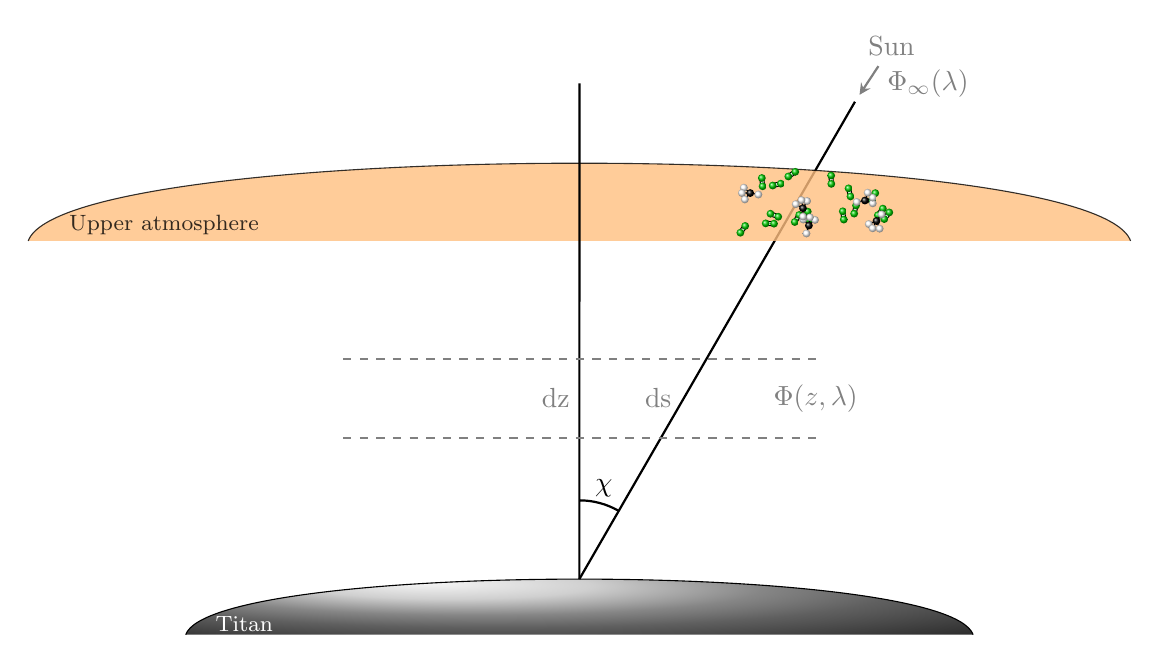
\begin{tikzpicture}[tight background]
\path[name path=incidence] (0,1) -- (0,-5);
\shadedraw[shading=ball,ball color=gray!50,name path=Titan surface] (-5,-5)  .. controls ++(70:1) and ++(110:1).. (5,-5)
        node[pos=0.1,below right=0pt,font=\footnotesize,inner sep=0.5pt,white]{Titan};
\draw[thick,name intersections={of=incidence and Titan surface}] (intersection-1) -- ++(60:7)
        coordinate[pin={[pin edge={stealth-,thick,shorten <=3pt},gray]85:Sun}] 
        node[gray,above right = -2pt and 8pt] {$\Phi_\infty(\lambda)$};
\draw[fill=orange!50,opacity=0.8] (-7,0) .. controls ++(70:1.4) and ++(110:1.4).. (7,0)
        node[pos=0.1,below right=0pt,font=\footnotesize,inner sep=0.5pt]{Upper atmosphere};
\draw[thick,name intersections={of=incidence and Titan surface}] (0,2) -- (intersection-1)
                                                                 ++(0,1) arc(90:60:1)
                                                                 (intersection-1)
                                                                 ++(75:1.2)node{$\chi$};
\draw[thick,dashed,gray]   (-3,-1.5) -- +(6,0)
                         ++(0,-1) -- +(6,0);
\node[left,gray] at (0,-2) {dz};
\node[gray] at (1,-2) {ds};
\node[gray] at (3,-2) {$\Phi(z,\lambda)$};
\foreach \ite in {1,...,15}
{
  \pgfmathparse{2+rnd*2}\let\xinit\pgfmathresult
  \pgfmathparse{rnd*0.9}\let\yinit\pgfmathresult
  \pgfmathparse{rnd*360}\let\ang\pgfmathresult
  \draw[shorten <=1.1pt,shorten >=1.1pt] (\xinit,\yinit)  -- ++(\ang:3pt);
  \draw[double=none,double distance=1pt] (\xinit,\yinit) node[N]{} -- ++(\ang:3pt) node[N]{};
}
\foreach \ite in {1,...,5}
{
  \pgfmathparse{2+rnd*2}\let\xinit\pgfmathresult
  \pgfmathparse{rnd*0.9}\let\yinit\pgfmathresult
  \pgfmathparse{rnd*360}\let\anginit\pgfmathresult
   \foreach \ang in {90,-120,-80,-30}
   {
     \pgfmathparse{\ang + \anginit}\let\angrel\pgfmathresult
     \draw (\xinit,\yinit) -- +(\angrel:3pt)node[H]{};
   }
  \draw (\xinit,\yinit)node[C]{};
}
\end{tikzpicture}
\end{document}
